\begin{enumerate}[label=\thesubsection.\arabic*, ref=\thesubsection.\theenumi]
	
	% Q.3
	\item 
	A $4 \times 4$ digital image has pixel intensities $\brak{U}$ as shown in the figure. The number of pixels with $U \le 4$ is:
	\hfill (DA~2025)
	\begin{figure}[H]
		\centering
		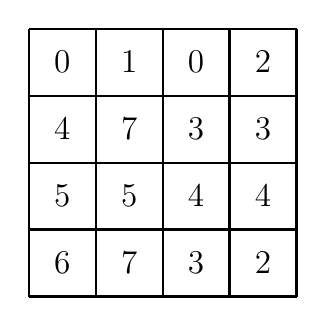
\begin{tikzpicture}[scale=0.85]
	\draw[thick] (0,0) grid (4,4);
	% Row 4 (top)
	\node at (0.5, 3.5) {\large 0};
	\node at (1.5, 3.5) {\large 1};
	\node at (2.5, 3.5) {\large 0};
	\node at (3.5, 3.5) {\large 2};
	% Row 3
	\node at (0.5, 2.5) {\large 4};
	\node at (1.5, 2.5) {\large 7};
	\node at (2.5, 2.5) {\large 3};
	\node at (3.5, 2.5) {\large 3};
	% Row 2
	\node at (0.5, 1.5) {\large 5};
	\node at (1.5, 1.5) {\large 5};
	\node at (2.5, 1.5) {\large 4};
	\node at (3.5, 1.5) {\large 4};
	% Row 1 (bottom)
	\node at (0.5, 0.5) {\large 6};
	\node at (1.5, 0.5) {\large 7};
	\node at (2.5, 0.5) {\large 3};
	\node at (3.5, 0.5) {\large 2};
\end{tikzpicture}
		\caption{Pixel Grid}
		\label{fig:DA-2025-3}
	\end{figure}
	\begin{enumerate}
		\begin{multicols}{4}
			\item $3$
			\item $8$
			\item $11$
			\item $9$
		\end{multicols}
	\end{enumerate}
	
	% Q.5
	\item 
	A rectangle has a length $L$ and a width $W$, where $L > W$. If the width, $W$, is increased by $10\%$, which one of the following statements is correct for all values of $L$ and $W$?
	\hfill (DA~2025)
	\begin{enumerate}
		\item Perimeter increases by $10\%$.
		\item Length of the diagonals increases by $10\%$.
		\item Area increases by $10\%$.
		\item The rectangle becomes a square.
	\end{enumerate}
	
	% Q.7
	\item 
	Weight of a person can be expressed as a function of their age. The function usually varies from person to person. Suppose this function is identical for two brothers, and it monotonically increases till the age of 50 years and then it monotonically decreases. Let $a_1$ and $a_2$ (in years) denote the ages of the brothers and $a_1 < a_2$. Which one of the following statements is correct about their age on the day when they attain the same weight?
	\hfill (DA~2025)
	\begin{enumerate}
		\begin{multicols}{2}
			\item $a_1 < a_2 < 50$
			\item $a_1 < 50 < a_2$
			\item $50 < a_1 < a_2$
			\item Either $a_1 = 50$ or $a_2 = 50$
		\end{multicols}
	\end{enumerate}
	
	% Q.9
	\item 
	If a real variable $x$ satisfies $3^{x^2} = 27 \times 9^x$, then the value of $\frac{2^{x^2}}{\brak{2^x}^2}$ is:
	\hfill (DA~2025)
	\begin{enumerate}
		\begin{multicols}{4}
			\item $2^{-1}$
			\item $2^0$
			\item $2^3$
			\item $2^{15}$
		\end{multicols}
	\end{enumerate}
	
	% Q.11
	\item 
	Suppose $X$ and $Y$ are random variables. The conditional expectation of $X$ given $Y$ is denoted by $E\sbrak{X \mid Y}$. Then $E\sbrak{E\sbrak{X \mid Y}}$ equals
	\hfill (DA~2025)
	\begin{enumerate}
		\begin{multicols}{4}
			\item $E\sbrak{X \mid Y}$
			\item $\frac{E\sbrak{X}}{E\sbrak{Y}}$
			\item $E\sbrak{X}$
			\item $E\sbrak{Y}$
		\end{multicols}
	\end{enumerate}
	
	% Q.12
	\item 
	The number of additions and multiplications involved in performing Gaussian elimination on any $n \times n$ upper triangular matrix is of the order
	\hfill (DA~2025)
	\begin{enumerate}
		\begin{multicols}{4}
			\item $O\brak{n}$
			\item $O\brak{n^2}$
			\item $O\brak{n^3}$
			\item $O\brak{n^4}$
		\end{multicols}
	\end{enumerate}
	
	% Q.13
	\item 
	The sum of the elements in each row of $\vec{A} \in \mathbb{R}^{n \times n}$ is 1. If $\vec{B} = \vec{A}^3 - 2\vec{A}^2 + \vec{A}$, which one of the following statements is correct (for $\vec{x} \in \mathbb{R}^n$)?
	\hfill (DA~2025)
	\begin{enumerate}
		\item The equation $\vec{Bx} = \vec{0}$ has no solution
		\item The equation $\vec{Bx} = \vec{0}$ has exactly two solutions
		\item The equation $\vec{Bx} = \vec{0}$ has infinitely many solutions
		\item The equation $\vec{Bx} = \vec{0}$ has a unique solution
	\end{enumerate}
	
	% Q.14
	\item 
	Let $f\brak{x} = \frac{e^x - e^{-x}}{2}, \; x \in \mathbb{R}$. Let $f^{(k)}\brak{a}$ denote the $k^{\text{th}}$ derivative of $f$ evaluated at $a$. What is the value of $f^{(10)}\brak{0}$? (Note: ! denotes factorial)
	\hfill (DA~2025)
	\begin{enumerate}
		\begin{multicols}{4}
			\item $0$
			\item $1$
			\item $\frac{1}{10!}$
			\item $\frac{2}{10!}$
		\end{multicols}
	\end{enumerate}
	
	% Q.17
	\item 
	Consider the following three relations:
	\begin{align*}
		&\text{Car } (\underline{\text{model}}, \underline{\text{year}}, \underline{\text{serial}}, \text{color}) \\
		&\text{Make } (\underline{\text{maker}}, \underline{\text{model}}) \\
		&\text{Own } (\underline{\text{owner}}, \underline{\text{serial}})
	\end{align*}
	A tuple in Car represents a specific car of a given model, made in a given year, with a serial number and a color. A tuple in Make specifies that a maker company makes cars of a certain model. A tuple in Own specifies that an owner owns the car with a given serial number. Keys are underlined; (owner, serial) together form key for Own. ($\bowtie$ denotes natural join)
	\begin{align}
		\pi_{\text{owner}}\brak{\text{Own} \bowtie \brak{\sigma_{\text{color} = \text{'red'}}\brak{\text{Car} \bowtie \brak{\sigma_{\text{maker} = \text{'ABC'}}\text{Make}}}}}
	\end{align}
	Which one of the following options describes what the above expression computes?
	\hfill (DA~2025)
	\begin{enumerate}
		\item All owners of a red car, a car made by ABC, or a red car made by ABC
		\item All owners of more than one car, where at least one car is red and made by ABC
		\item All owners of a red car made by ABC
		\item All red cars made by ABC
	\end{enumerate}
	
	% Q.18
	\item 
	Consider a hash table of size 10 with indices $\cbrak{0, 1, \dots, 9}$, with the hash function
	\begin{align}
		h\brak{x} = 3x \brak{\text{mod } 10}
	\end{align}
	where linear probing is used to handle collisions. The hash table is initially empty and then the following sequence of keys is inserted into the hash table: $1, 4, 5, 6, 14, 15$. The indices where the keys 14 and 15 are stored are, respectively
	\hfill (DA~2025)
	\begin{enumerate}
		\begin{multicols}{4}
			\item 2 and 5
			\item 2 and 6
			\item 4 and 5
			\item 4 and 6
		\end{multicols}
	\end{enumerate}
	
	% Q.19
	\item 
	Let $X$ be a continuous random variable whose cumulative distribution function (CDF) $F_X\brak{x}$, for some $t$, is given as follows:
	\begin{align}
		F_X\brak{x} = \begin{cases}
			0 & x \le t \\
			\frac{x - t}{4 - t} & t \le x \le 4 \\
			1 & x \ge 4
		\end{cases}
	\end{align}
	If the median of $X$ is 3, then what is the value of $t$?
	\hfill (DA~2025)
	\begin{enumerate}
		\begin{multicols}{4}
			\item $2$
			\item $1$
			\item $-1$
			\item $0$
		\end{multicols}
	\end{enumerate}
	
	% Q.20
	\item 
	Let $X = aZ + b$, where $Z$ is a standard normal random variable, and $a, b$ are two unknown constants. It is given that
	\begin{align}
		E\sbrak{X} = 1, \quad E\sbrak{\brak{X - E\sbrak{X}}Z} = -2, \quad E\sbrak{\brak{X - E\sbrak{X}}^2} = 4,
	\end{align}
	where $E\sbrak{X}$ denotes the expectation of random variable $X$. The values of $a, b$ are:
	\hfill (DA~2025)
	\begin{enumerate}
		\begin{multicols}{2}
			\item $a = -2, \; b = 1$
			\item $a = 2, \; b = -1$
			\item $a = -2, \; b = -1$
			\item $a = 1, \; b = 1$
		\end{multicols}
	\end{enumerate}
	
	% Q.21
	\item 
	It is given that $P\brak{X \ge 2} = 0.25$ for an exponentially distributed random variable $X$ with $E\sbrak{X} = \frac{1}{\lambda}$, where $E\sbrak{X}$ denotes the expectation of $X$. What is the value of $\lambda$? ($\ln$ denotes natural logarithm)
	\hfill (DA~2025)
	\begin{enumerate}
		\begin{multicols}{4}
			\item $\ln 2$
			\item $\ln 4$
			\item $\ln 3$
			\item $\ln 0.25$
		\end{multicols}
	\end{enumerate}
	
	% Q.23
	\item 
	Consider the following Python declarations of two lists.
	\begin{lstlisting}[frame=single, basicstyle=\rmfamily]
A = [1, 2, 3]
B = [4, 5, 6]
	\end{lstlisting}
	Which one of the following statements results in $A = [1, 2, 3, 4, 5, 6]$?
	\hfill (DA~2025)
	\begin{enumerate}
		\begin{multicols}{4}
			\item \lstinline|A.extend(B)|
			\item \lstinline|A.append(B)|
			\item \lstinline|A.update(B)|
			\item \lstinline|A.insert(B)|
		\end{multicols}
	\end{enumerate}
	
	% Q.24
	\item 
	Consider two functions $f: \mathbb{R} \to \mathbb{R}$ and $g: \mathbb{R} \to \brak{1, \infty}$. Both functions are differentiable at a point $c$. Which of the following functions is/are ALWAYS differentiable at $c$? The symbol $\cdot$ denotes product and the symbol $\circ$ denotes composition of functions.
	\hfill (DA~2025)
	\begin{enumerate}
		\begin{multicols}{4}
			\item $f \pm g$
			\item $f \cdot g$
			\item $\frac{f}{g}$
			\item $f \circ g + g \circ f$
		\end{multicols}
	\end{enumerate}
	
	% Q.25
	\item 
	Which of the following statements is/are correct?
	\hfill (DA~2025)
	\begin{enumerate}
		\item $\mathbb{R}^n$ has a unique set of orthonormal basis vectors
		\item $\mathbb{R}^n$ does not have a unique set of orthonormal basis vectors
		\item Linearly independent vectors in $\mathbb{R}^n$ are orthonormal
		\item Orthonormal vectors in $\mathbb{R}^n$ are linearly independent
	\end{enumerate}
	
	% Q.27
	\item 
	For which of the following inputs does binary search take time $O\brak{\log n}$ in the worst case?
	\hfill (DA~2025)
	\begin{enumerate}
		\item An array of $n$ integers in any order
		\item A linked list of $n$ integers in any order
		\item An array of $n$ integers in increasing order
		\item A linked list of $n$ integers in increasing order
	\end{enumerate}
	
	% Q.28
	\item 
	Let $\vec{A} = \vec{I}_n + \vec{x}\vec{x}^{\top}$ where $\vec{I}_n$ is the $n \times n$ identity matrix and $\vec{x} \in \mathbb{R}^n$, $\vec{x}^{\top}\vec{x} = 1$. Which of the following options is/are correct?
	\hfill (DA~2025)
	\begin{enumerate}
		\item Rank of $\vec{A}$ is $n$
		\item $\vec{A}$ is invertible
		\item $0$ is an eigenvalue of $\vec{A}$
		\item $\vec{A}^{-1}$ has a negative eigenvalue
	\end{enumerate}
	
	% Q.29
	\item 
	Suppose that insertion sort is applied to the array $\sbrak{1, 3, 5, 7, 9, 11, x, 15, 13}$ and it takes exactly two swaps to sort the array. Select all possible values of $x$.
	\hfill (DA~2025)
	\begin{enumerate}
		\begin{multicols}{4}
			\item $10$
			\item $12$
			\item $14$
			\item $16$
		\end{multicols}
	\end{enumerate}
	
	% Q.31
	\item 
	There are three boxes containing white balls and black balls.
	\begin{itemize}
		\item Box-1 contains 2 black and 1 white balls.
		\item Box-2 contains 1 black and 2 white balls.
		\item Box-3 contains 3 black and 3 white balls.
	\end{itemize}
	In a random experiment, one of these boxes is selected, where the probability of choosing Box-1 is $\frac{1}{2}$, Box-2 is $\frac{1}{6}$, and Box-3 is $\frac{1}{3}$. A ball is drawn at random from the selected box. Given that the ball drawn is white, the probability that it is drawn from Box-2 is \underline{\hspace{1.5cm}}.
	\hfill (DA~2025)
	
	% Q.32
	\item 
	$\lim\limits_{t \to +\infty} \sqrt{t^2 + t} - t = \underline{\hspace{1.5cm}}$.
	\hfill (DA~2025)
	
	% Q.33
	\item 
	On a relation named Loan of a bank:
	\begin{figure}[H]
		\centering
		\begin{tabular}{|c|c|c|}
	\hline
	\textbf{loan\_number} & \textbf{branch\_name} & \textbf{amount} \\ \hline
	L11 & Banjara Hills & 90000 \\ \hline
	L14 & Kondapur      & 50000 \\ \hline
	L15 & SR Nagar      & 40000 \\ \hline
	L22 & SR Nagar      & 25000 \\ \hline
	L23 & Balanagar     & 80000 \\ \hline
	L25 & Kondapur      & 70000 \\ \hline
	L19 & SR Nagar      & 65000 \\ \hline
\end{tabular}
		\caption{}
		\label{fig:DA-2025-33}
	\end{figure}
	the following SQL query is executed.
	\begin{lstlisting}[frame=single, basicstyle=\rmfamily]
SELECT L1.loan_number
FROM Loan L1
WHERE L1.amount > (SELECT MAX (L2.amount)
	FROM Loan L2
	WHERE L2.branch_name = 'SR Nagar');
	\end{lstlisting}
	The number of rows returned by the query is \underline{\hspace{1.5cm}}.
	\hfill (DA~2025)
	
	% Q.34
	\item 
	Given data $\cbrak{\brak{-1, 1}, \brak{2, 5}, \brak{3, 5}}$ of the form $\brak{x, y}$, we fit a model $y = wx$ using linear least-squares regression. The optimal value of $w$ is \underline{\hspace{1.5cm}}.
	\hfill (DA~2025)
	

	% Q.35
	\item 
	The naive Bayes classifier is used to solve a two-class classification problem with class-labels $y_1, y_2$. Suppose the prior probabilities are $P\brak{y_1} = \frac{1}{3}$ and $P\brak{y_2} = \frac{2}{3}$. Assuming a discrete feature space with
	\begin{align}
		P\brak{\vec{x} \mid y_1} = \frac{3}{4} \quad \text{and} \quad P\brak{\vec{x} \mid y_2} = \frac{1}{4}
	\end{align}
	for a specific feature vector $\vec{x}$. The probability of misclassifying $\vec{x}$ is \underline{\hspace{1.5cm}}.
	\hfill (DA~2025)
	% Q.36
	\item 
	Let $Y = Z^2, \; Z = \frac{X - \mu}{\sigma}$, where $X$ is a normal random variable with mean $\mu$ and variance $\sigma^2$. The variance of $Y$ is
	\hfill (DA~2025)
	\begin{enumerate}
		\begin{multicols}{4}
			\item $1$
			\item $2$
			\item $3$
			\item $4$
		\end{multicols}
	\end{enumerate}
	
	% Q.37
	\item 
	Let $\vec{A} \in \mathbb{R}^{n \times n}$ be such that $\vec{A}^3 = \vec{A}$. Which one of the following statements is ALWAYS correct?
	\hfill (DA~2025)
	\begin{enumerate}
		\item $\vec{A}$ is invertible
		\item Determinant of $\vec{A}$ is 0
		\item The sum of the diagonal elements of $\vec{A}$ is 1
		\item $\vec{A}$ and $\vec{A}^2$ have the same rank
	\end{enumerate}
	
	% Q.38
	\item 
	Let $\cbrak{\vec{x}_1, \vec{x}_2, \dots, \vec{x}_n}$ be a set of linearly independent vectors in $\mathbb{R}^n$. Let the $(i, j)$-th element of matrix $\vec{A} \in \mathbb{R}^{n \times n}$ be given by $A_{ij} = \vec{x}_i^{\top}\vec{x}_j, \; 1 \le i, j \le n$. Which one of the following statements is correct?
	\hfill (DA~2025)
	\begin{enumerate}
		\item $\vec{A}$ is invertible
		\item 0 is a singular value of $\vec{A}$
		\item Determinant of $\vec{A}$ is 0
		\item $\vec{z}^{\top}\vec{A}\vec{z} = 0$ for some non-zero $\vec{z} \in \mathbb{R}^n$
	\end{enumerate}
	
	% Q.39
	\item 
	Consider the cumulative distribution function (CDF) of a random variable $X$:
	\begin{align}
		F_X\brak{x} = \begin{cases}
			0 & x \le -1 \\
			\frac{1}{4}\brak{x + 1}^2 & -1 \le x \le 1 \\
			1 & x \ge 1
		\end{cases}
	\end{align}
	The value of $P\brak{X^2 \le 0.25}$ is
	\hfill (DA~2025)
	\begin{enumerate}
		\begin{multicols}{4}
			\item $0.625$
			\item $0.25$
			\item $0.5$
			\item $0.5625$
		\end{multicols}
	\end{enumerate}
	
	% Q.40
	\item 
	A random variable $X$ is said to be distributed as $\text{Bernoulli}(\theta)$, denoted by $X \sim \text{Bernoulli}(\theta)$, if $P\brak{X = 1} = \theta, \; P\brak{X = 0} = 1 - \theta$ for $0 < \theta < 1$. Let $Y = \sum_{i=1}^{300} X_i$, where $X_i \sim \text{Bernoulli}(\theta), \; i = 1, 2, \dots, 300$ be independent and identically distributed random variables with $\theta = 0.25$. The value of $P\brak{60 \le Y \le 90}$ after approximation through Central Limit Theorem, is given by (Recall that $\phi\brak{x} = \frac{1}{\sqrt{2\pi}}\int_{-\infty}^x e^{-\frac{t^2}{2}}\,dt$)
	\hfill (DA~2025)
	\begin{enumerate}
		\begin{multicols}{2}
			\item $\phi\brak{2} - \phi\brak{-2}$
			\item $\phi\brak{1} - \phi\brak{-1}$
			\item $\phi\brak{3} - \phi\brak{-3}$
			\item $\phi\brak{90} - \phi\brak{60}$
		\end{multicols}
	\end{enumerate}
	
	% Q.41
	\item 
	For $x \in \mathbb{R}$, the floor function is denoted by $f\brak{x} = \lfloor x \rfloor$ and defined as follows
	\begin{align}
		\lfloor x \rfloor = k, \quad k \le x < k + 1
	\end{align}
	where $k$ is an integer. Let $Y = \lfloor X \rfloor$ where $X$ is an exponentially distributed random variable with mean $\frac{1}{\ln 10}$, where $\ln$ denotes natural logarithm. For any positive integer $l$, one can write the probability of the event $Y = l$ as follows
	\begin{align}
		P\brak{Y = l} = q^l\brak{1 - q}
	\end{align}
	The value of $q$ is
	\hfill (DA~2025)
	\begin{enumerate}
		\begin{multicols}{4}
			\item $0.1$
			\item $0.01$
			\item $0.5$
			\item $0.434$
		\end{multicols}
	\end{enumerate}
	
	% Q.45
	\item 
	A random experiment consists of throwing 100 fair dice, each die having six faces numbered 1 to 6. An event $A$ represents the set of all outcomes where at least one of the dice shows a 1. Then, $P\brak{A} = $
	\hfill (DA~2025)
	\begin{enumerate}
		\begin{multicols}{4}
			\item $0$
			\item $1$
			\item $\brak{\frac{5}{6}}^{100}$
			\item $1 - \brak{\frac{5}{6}}^{100}$
		\end{multicols}
	\end{enumerate}
	
	% Q.47
	\item 
	Consider the following Python code snippet.
	\begin{lstlisting}[frame=single, basicstyle=\rmfamily]
A = {"this", "that"}
B = {"that", "other"}
C = {"other", "this"}
while "other" in C:
	if "this" in A:
		A, B, C = A - B, B - C, C - A
	if "that" in B:
		A, B, C = C | A, A | B, B | C
	\end{lstlisting}
	When the above program is executed, at the end, which of the following sets contains ``this''?
	\hfill (DA~2025)
	\begin{enumerate}
		\begin{multicols}{4}
			\item Only A
			\item Only B
			\item Only C
			\item A, C
		\end{multicols}
	\end{enumerate}
	
	% Q.49
	\item 
	Consider the function
	\begin{align}
		f\brak{x} = \frac{x^3}{3} + \frac{7}{2}x^2 + 10x + \frac{133}{2}, \quad x \in \sbrak{-8, 0}
	\end{align}
	Which of the following statements is/are correct?
	\hfill (DA~2025)
	\begin{enumerate}
		\item The maximum value of $f$ is attained at $x = -5$
		\item The minimum value of $f$ is attained at $x = -2$
		\item The maximum value of $f$ is $\frac{133}{2}$
		\item The minimum value of the derivative of $f$ is attained at $x = -\frac{7}{2}$
	\end{enumerate}
	
	% Q.50
	\item 
	Let $\vec{x}_1, \vec{x}_2, \vec{x}_3, \vec{x}_4, \vec{x}_5$ be a system of orthonormal vectors in $\mathbb{R}^{10}$. Consider the matrix $\vec{A} = \vec{x}_1\vec{x}_1^{\top} + \dots + \vec{x}_5\vec{x}_5^{\top}$. Which of the following statements is/are correct?
	\hfill (DA~2025)
	\begin{enumerate}
		\item Singular values of $\vec{A}$ are also its eigenvalues
		\item Singular values of $\vec{A}$ are either 0 or 1
		\item Determinant of $\vec{A}$ is 1
		\item $\vec{A}$ is invertible
	\end{enumerate}
	
	% Q.51
	\item 
	Let $f: \mathbb{R} \to \mathbb{R}$ be a twice-differentiable function and suppose its second derivative satisfies $f''\brak{x} > 0$ for all $x \in \mathbb{R}$. Which of the following statements is/are ALWAYS correct?
	\hfill (DA~2025)
	\begin{enumerate}
		\item $f$ has a local minima
		\item There does not exist $x$ and $y$, $x \ne y$ such that $f'\brak{x} = f'\brak{y} = 0$
		\item $f$ has at most one global minimum
		\item $f$ has at most one local minimum
		
	\end{enumerate}
	
	% Q.52
	\item 
	An $n \times n$ matrix $\vec{A}$ with real entries satisfies the property: $\norm{\vec{Ax}}^2 = \norm{\vec{x}}^2$, for all $\vec{x} \in \mathbb{R}^n$, where $\norm{\cdot}$ denotes the Euclidean norm. Which of the following statements is/are ALWAYS correct?
	\hfill (DA~2025)
	\begin{enumerate}
		\item $\vec{A}$ must be orthogonal
		\item $\vec{A} = \vec{I}$ where $\vec{I}$ denotes the identity matrix, is the only solution
		\item The eigenvalues of $\vec{A}$ are either +1 or -1
		\item $\vec{A}$ has full rank
	\end{enumerate}
	
	% Q.53
	\item 
	Consider designing a linear binary classifier $f\brak{\vec{x}} = \text{sign}\brak{\vec{w}^{\top}\vec{x} + b}, \; \vec{x} \in \mathbb{R}^2$ on the following training data:
	\begin{align}
		\text{Class-1}: \cbrak{\myvec{2 \\ 0}, \myvec{0 \\ 2}, \myvec{2 \\ 2}}, \quad \text{Class-2}: \cbrak{\myvec{0 \\ 0}}
	\end{align}
	Hard-margin support vector machine (SVM) formulation is solved to obtain $\vec{w}$ and $b$. Which of the following options is/are correct?
	\hfill (DA~2025)
	\begin{enumerate}
		\item $\vec{w} = \myvec{4 \\ 4}$ and $b = 1$
		\item The number of support vectors is 3
		\item The margin is $\sqrt{2}$
		\item Training accuracy is 98\%
		
	\end{enumerate}
	
	% Q.54
	\item 
	Consider a coin-toss experiment where the probability of head showing up is $p$. In the $i^{\text{th}}$ coin toss, let $X_i = 1$ if head appears, and $X_i = 0$ if tail appears. Consider
	\begin{align}
		\hat{p} = \frac{1}{n}\sum_{i=1}^n X_i
	\end{align}
	where $n$ is the total number of independent coin tosses. Which of the following statements is/are correct?
	\hfill (DA~2025)
	\begin{enumerate}
		\item $E\sbrak{\hat{p}} = p$
		\item $E\sbrak{\hat{p}} = \frac{p}{n}$
		\item As $n$ increases, variance of $\hat{p}$ decreases
		\item Variance of $\hat{p}$ does not depend on $n$
	\end{enumerate}
	
	% Q.58
	\item 
	Let $G$ be a simple, unweighted, and undirected graph. A subset of the vertices and edges of $G$ are shown below.
	\begin{figure}[H]
		\centering
		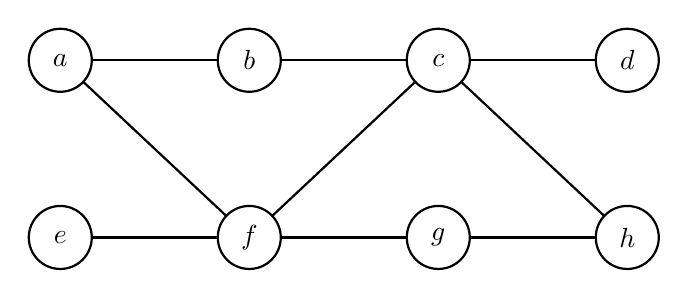
\begin{tikzpicture}[scale=1.5, >=stealth, every node/.style={circle, draw, thick, minimum size=8mm, inner sep=0pt}]
	% Top Row Vertices
	\coordinate (a) at (0, 1.5);
	\coordinate (b) at (1.6, 1.5);
	\coordinate (c) at (3.2, 1.5);
	\coordinate (d) at (4.8, 1.5);
	
	% Bottom Row Vertices
	\coordinate (e) at (0, 0);
	\coordinate (f) at (1.6, 0);
	\coordinate (g) at (3.2, 0);
	\coordinate (h) at (4.8, 0);
	
	% Edges
	\draw[thick] (0, 1.5) -- (1.6, 1.5); % a - b
	\draw[thick] (1.6, 1.5) -- (3.2, 1.5); % b - c
	\draw[thick] (3.2, 1.5) -- (4.8, 1.5); % c - d
	
	\draw[thick] (0, 0) -- (1.6, 0); % e - f
	\draw[thick] (1.6, 0) -- (3.2, 0); % f - g
	\draw[thick] (3.2, 0) -- (4.8, 0); % g - h
	
	\draw[thick] (0, 1.5) -- (1.6, 0); % a - f
	\draw[thick] (1.6, 0) -- (3.2, 1.5); % f - c
	\draw[thick] (3.2, 1.5) -- (4.8, 0); % c - h
	
	% Nodes drawn on top of lines
	\node[fill=white] at (a) {$a$};
	\node[fill=white] at (b) {$b$};
	\node[fill=white] at (c) {$c$};
	\node[fill=white] at (d) {$d$};
	
	\node[fill=white] at (e) {$e$};
	\node[fill=white] at (f) {$f$};
	\node[fill=white] at (g) {$g$};
	\node[fill=white] at (h) {$h$};
	\end{tikzpicture}
		\caption{}
		\label{fig:DA-2025-58}
	\end{figure}
	It is given that $a-b-c-d$ is a shortest path between $a$ and $d$; $e-f-g-h$ is a shortest path between $e$ and $h$; $a-f-c-h$ is a shortest path between $a$ and $h$. Which of the following is/are NOT the edges of $G$?
	\hfill (DA~2025)
	\begin{enumerate}
		\begin{multicols}{4}
			\item $\brak{b, d}$
			\item $\brak{b, g}$
			\item $\brak{b, h}$
			\item $\brak{e, g}$
		\end{multicols}
	\end{enumerate}
	
	% Q.59
	\item 
	Let $f: \mathbb{R} \to \mathbb{R}$ be such that $\abs{f\brak{x} - f\brak{y}} \le \brak{x - y}^2$ for all $x, y \in \mathbb{R}$. Then
	\begin{align}
		f\brak{1} - f\brak{0} = \underline{\hspace{1.5cm}}
	\end{align}
	\hfill (DA~2025)
	
	% Q.60
	\item 
	Let $D = \cbrak{\vec{x}^{(1)}, \dots, \vec{x}^{(n)}}$ be a dataset of $n$ observations where each $\vec{x}^{(i)} \in \mathbb{R}^{100}$. It is given that $\sum_{i=1}^n \vec{x}^{(i)} = \vec{0}$. The covariance matrix computed from $D$ has eigenvalues $\lambda_i = 100^{2-i}, \; 1 \le i \le 100$. Let $\vec{u} \in \mathbb{R}^{100}$ be the direction of maximum variance with $\vec{u}^{\top}\vec{u} = 1$. The value of
	\begin{align}
		\frac{1}{n}\sum_{i=1}^n \brak{\vec{u}^{\top}\vec{x}^{(i)}}^2 = \underline{\hspace{1.5cm}}
	\end{align}
	\hfill (DA~2025)
	
	% Q.61
	\item 
	A bag contains 5 white balls and 10 black balls. In a random experiment, $n$ balls are drawn from the bag one at a time with replacement. Let $S_n$ denote the total number of black balls drawn in the experiment.
	The expectation of $S_{100}$ denoted by $E\sbrak{S_{100}} = \underline{\hspace{1.5cm}}$.
	\hfill (DA~2025)
	
	% Q.62
	\item 
	Consider the following tables, Loan and Borrower, of a bank.
	\begin{figure}[H]
		\centering
		\begin{minipage}[t]{0.52\textwidth}
	\centering
	\textbf{Loan} \\[1ex]
	\begin{tabular}{|c|c|c|}
		\hline
		\textbf{loan\_num} & \textbf{branch\_name} & \textbf{amount} \\ \hline
		L11 & Banjara Hills & 90000 \\ \hline
		L14 & Kondapur      & 50000 \\ \hline
		L15 & SR Nagar      & 40000 \\ \hline
		L22 & SR Nagar      & 25000 \\ \hline
		L23 & Balanagar     & 80000 \\ \hline
		L25 & Kondapur      & 70000 \\ \hline
		L19 & SR Nagar      & 65000 \\ \hline
	\end{tabular}
\end{minipage}%
\begin{minipage}[t]{0.45\textwidth}
	\centering
	\textbf{Borrower} \\[1ex]
	\begin{tabular}{|c|c|}
		\hline
		\textbf{customer\_name} & \textbf{loan\_num} \\ \hline
		Anand   & L11 \\ \hline
		Karteek & L11 \\ \hline
		Karteek & L14 \\ \hline
		Ankita  & L15 \\ \hline
		Gopal   & L19 \\ \hline
		Karteek & L22 \\ \hline
		Karteek & L23 \\ \hline
		Sunil   & L23 \\ \hline
		Sunil   & L25 \\ \hline
	\end{tabular}
\end{minipage}
		\caption{}
		\label{fig:DA-2025-62}
	\end{figure}
	Query: $\pi_{\text{branch\_name}, \text{customer\_name}}(\text{Loan} \bowtie \text{Borrower}) \div \pi_{\text{branch\_name}}(\text{Loan})$
	where $\bowtie$ denotes natural join.
	The number of tuples returned by the above relational algebra query is \underline{\hspace{1.5cm}}.
	\hfill (DA~2025)
	
	% Q.63
	\item 
	Consider the following Python code snippet.
	\begin{lstlisting}[frame=single, basicstyle=\rmfamily]
def f(a, b):
	if (a == 0):
		return b
	if (a % 2 == 1):
		return 2 * f((a - 1) / 2, b)
	return b + f(a - 1, b)
	
print(f(15, 10))
	\end{lstlisting}
	The value printed by the code snippet is \underline{\hspace{1.5cm}}.
	\hfill (DA~2025)
	
	% Q.64
	\item 
	Consider the following pseudocode.
	\begin{lstlisting}[frame=single, basicstyle=\rmfamily]
Create empty stack S
Set x = 0, flag = 0, sum = 0
Push x onto S

while (S is not empty) {
	if (flag equals 0){
		Set x = x + 1
		Push x onto S
	}
	if (x equals 8):
		Set flag = 1
		if (flag equals 1){
			x = Pop(S)
			if (x is odd):
			Pop(S)
			Set sum = sum + x
	}
}
Output sum
	\end{lstlisting}
	The value of sum output by a program executing the above pseudocode is \underline{\hspace{1.5cm}}.
	\hfill (DA~2025)
	
	% Q.65
	\item 
	Consider a directed graph $G = (V, E)$, where $V = \{0, 1, 2, \dots, 100\}$ and $E = \{(i, j) : 0 < j - i \le 2 \text{ for all } i, j \in V\}$. Suppose the adjacency list of each vertex is in decreasing order of vertex number, and depth-first search (DFS) is performed at vertex 0. The number of vertices that will be discovered after vertex 50 is \underline{\hspace{1.5cm}}.
	\hfill (DA~2025)
	
\end{enumerate}